% Created 2019-11-20 三 11:44
\documentclass[11pt]{article}
\usepackage[utf8]{inputenc}
\usepackage[T1]{fontenc}
\usepackage{fixltx2e}
\usepackage{graphicx}
\usepackage{longtable}
\usepackage{float}
\usepackage{wrapfig}
\usepackage{rotating}
\usepackage[normalem]{ulem}
\usepackage{amsmath}
\usepackage{textcomp}
\usepackage{marvosym}
\usepackage{wasysym}
\usepackage{amssymb}
\usepackage{hyperref}
\tolerance=1000
\author{iwos-ml}
\date{\today}
\title{iwos\_flink流数据处理}
\hypersetup{
  pdfkeywords={},
  pdfsubject={},
  pdfcreator={Emacs 25.3.1 (Org mode 8.2.10)}}
\begin{document}

\maketitle
\tableofcontents

\section{部署}
\label{sec-1}
\begin{itemize}
\item docker
\begin{itemize}
\item 查看flink-deploy
\end{itemize}
\item checkpoint
\begin{itemize}
\item 需要在代码中配置(\href{https://github.com/apache/flink-playgrounds/blob/master/docker/ops-playground-image/java/flink-playground-clickcountjob/src/main/java/org/apache/flink/playgrounds/ops/clickcount/ClickEventCount.java}{参考代码java})
\item \href{https://ci.apache.org/projects/flink/flink-docs-release-1.9/zh/ops/state/checkpoints.html}{docs}
\end{itemize}
\item savepoint
\begin{itemize}
\item \href{https://ci.apache.org/projects/flink/flink-docs-release-1.9/zh/ops/state/savepoints.html}{docs}
\end{itemize}
\end{itemize}


\section{应用开发}
\label{sec-2}
\begin{itemize}
\item 说明
\begin{itemize}
\item 微服务
\item 编程语言, java, python都可以, java文档更全
\end{itemize}
\item 编程语言
\begin{itemize}
\item java
\begin{itemize}
\item \href{https://ci.apache.org/projects/flink/flink-docs-release-1.9/zh/dev/projectsetup/java_api_quickstart.html}{项目构建设置docs}
\end{itemize}
\item python
\begin{itemize}
\item \href{https://ci.apache.org/projects/flink/flink-docs-release-1.9/zh/flinkDev/building.html#build-pyflink}{构建pyflink}
\begin{itemize}
\item 编程模型使用的抽象级别为:tableAPI
\end{itemize}
\item 特别说明:如果需要安装新版的pyflink必须使用上面的说明,pip安装的是1.0版本
\end{itemize}
\end{itemize}
\item 编程模型抽象级别的挑选
\begin{itemize}
\item 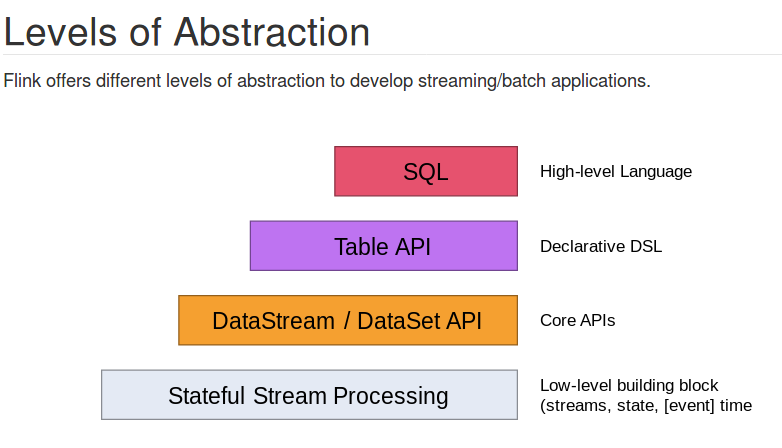
\includegraphics[width=.9\linewidth]{./material/编程模型抽象级别.png}
\end{itemize}
\end{itemize}
% Emacs 25.3.1 (Org mode 8.2.10)
\end{document}
